\documentclass{article}

% Use the preprint option for arXiv-friendly title block (no "Submitted to NeurIPS..." banner).
\usepackage[preprint]{neurips_2024}

\usepackage[utf8]{inputenc}
\usepackage[T1]{fontenc}
\usepackage{microtype}
\usepackage{booktabs}
\usepackage{graphicx}
\usepackage{amsmath, amssymb}
\usepackage{listings}
\usepackage{xcolor}
\usepackage{url}
\usepackage{hyperref}
\hypersetup{colorlinks=true, citecolor=blue, urlcolor=blue, linkcolor=blue}
\usepackage[capitalize,noabbrev]{cleveref}

% --- Listings style for Python / SQL / text -----------------------------------
\definecolor{codebg}{rgb}{0.97,0.97,0.97}
\definecolor{codecomment}{rgb}{0.25,0.5,0.35}
\definecolor{codekeyword}{rgb}{0.0,0.35,0.7}
\definecolor{codestring}{rgb}{0.6,0.2,0.2}

\lstdefinestyle{paperstyle}{
  backgroundcolor=\color{codebg},
  basicstyle=\small\ttfamily,
  commentstyle=\color{codecomment}\itshape,
  keywordstyle=\color{codekeyword}\bfseries,
  stringstyle=\color{codestring},
  numberstyle=\tiny\color{gray},
  numbers=left,
  numbersep=6pt,
  frame=single,
  framesep=4pt,
  rulecolor=\color{black!20},
  breaklines=true,
  breakatwhitespace=true,
  tabsize=2,
  showstringspaces=false,
  captionpos=b,
  xleftmargin=10pt,
  xrightmargin=4pt,
}
\lstset{style=paperstyle}

% --- Title block --------------------------------------------------------------
\title{Cross-Judge Validation and Multi-Track Prompt Iteration\\for AI Agent Memory Systems}

\author{%
  Peter J.\ Medina\\
  HeurChain\\
  \texttt{peter@carlssoncreative.com}\\
}

\begin{document}
\maketitle

\begin{abstract}
We report findings from iterative prompt-engineering of HeurChain, a hybrid (BM25 + dense bge-m3) memory broker for AI agents, evaluated on LongMemEval-S \citep{longmemeval_2025}. We make three methodological contributions. First, we propose \emph{cross-frontier per-question judge agreement} as a defensibility metric for LLM-as-judge benchmarking: by re-judging an identical cache of retrieved facts with two independent frontier judges (DeepSeek V3.1 671B and Kimi K2.6), we measure 87.8\% per-question agreement across 180 questions, and we use the residual disagreement to localize same-class judge bias to between 1 and 7 percentage points of inflation per category. Second, we describe a \emph{multi-track Karpathy iteration cycle} over a benchmark harness in which extraction, answering, and retrieval are iterated as independent tracks; we show that a null result on extraction iteration (v4, 1/22 wins on temporal-reasoning failures) can be misleading, that 25 minutes of answer-prompt iteration (v4a then v4b) recovers an additional 6/22 wins, and that a subsequent retrieval-side iteration (v4c, a graph-lite event index over haystack-wide re-extracted facts) recovers a further 3/12 wins on the retrieval-miss residual --- bringing the cumulative cascade to \textbf{10/22 (45.5\%)} on the previously failing items, or a projected $+33$\,pp lift on the full temporal-reasoning category with no model retraining. We further report that, in the v4c stage, dumping ALL relevant facts (60-fact context) produced 0/12 wins while a 20-fact event-indexed selection produced 3/12, providing direct evidence that \emph{selection dominates recall} once retrieval has surfaced the answer-bearing session. Third, we define a \texttt{fact\_contains\_gold} diagnostic that exposes cases where Hit@10 is high but the extracted facts do not contain the answer-bearing detail. We release the full harness and per-record results.
\end{abstract}

\section{Introduction}
\label{sec:intro}

A growing line of work on long-horizon AI agents treats \emph{memory} as a first-class system: Mem0 \citep{mem0_2025}, Zep / Graphiti \citep{zep_2025}, and Letta / MemGPT \citep{memgpt_2023} each propose distinct architectures for storing, updating, and retrieving facts across many conversations. The dominant benchmark for evaluating these systems is LongMemEval-S \citep{longmemeval_2025}, which scores an end-to-end pipeline (retrieval + answer generation + LLM judging) on 500 long-context questions across six reasoning categories.

Two methodological problems are common in this evaluation regime. First, \textbf{same-class judge bias}: when the answer model and the judge model are drawn from the same model family (or, in the most extreme case, are the same model), the judge tends to accept ``close enough'' answers of exactly the shape the answerer naturally produces \citep{llm_judge_2023}. Second, \textbf{the gap between retrieval Hit@k and answerability}: a question can have its gold-bearing session retrieved in top-$k$ while the \emph{facts} extracted from that session never contain the answer. Retrieval metrics alone do not surface this failure mode.

In this paper we report findings from iterating HeurChain's fact-extraction and answer prompts across three versions (v2 baseline $\to$ v3 structured-content unpacking $\to$ v4 ISO date tagging, with v4a/v4b answer-side variants). Along the way we develop tooling that addresses both problems above:

\begin{enumerate}
  \item A \textbf{cross-judge methodology} that fixes the retrieved facts and varies only the answer + judge model, allowing per-question comparison of judge verdicts at near-zero marginal cost ($\sim$1 hour wall time using free Ollama Cloud credits).
  \item A \textbf{multi-track prompt iteration cycle} in which extraction, answer, and retrieval are independent iteration tracks; we show that the v4 extraction prompt produced a null result in isolation, the combined v4 + v4b answer prompt recovered $+27.3$\,pp on the targeted failure set, and a subsequent v4c retrieval-side iteration (haystack-wide re-extraction plus a graph-lite event index) brought the cumulative cascade to 45.5\%. All three tracks required independent iteration; single-track methodology would have terminated at the v4 null.
  \item A \texttt{fact\_contains\_gold} diagnostic that flags questions where retrieval succeeded (the gold session is in top-$k$) but extraction destroyed the answer-bearing detail.
\end{enumerate}

Our results are intentionally hedged: each per-category measurement uses 30 tasks (180 tasks total), the answerer is a 14B parameter local model rather than a frontier model, and we measure only one product. We emphasize methodology as the primary contribution.

\section{Background and Related Work}
\label{sec:related}

\textbf{Mem0} \citep{mem0_2025} introduces a memory layer that distills conversations into facts with explicit update operations, reporting strong QA accuracy on LongMemEval with GPT-4o as the judge. Their evaluation uses GPT-4o for both the answerer and the judge --- an in-family pairing that motivates our cross-judge analysis.

\textbf{Zep / Graphiti} \citep{zep_2025} proposes a temporal knowledge graph for memory, with explicit edge timestamps used for time-aware retrieval. Their architecture inspires our v4c proposal for an event index (\Cref{sec:future}).

\textbf{Letta / MemGPT} \citep{memgpt_2023} frames memory as an OS-like virtual context with self-managed paging. Their evaluation reports document-QA scores; LongMemEval was introduced after their original publication.

\textbf{LongMemEval-S} \citep{longmemeval_2025} is the dataset we use: 500 questions across six reasoning categories (single-session-user, single-session-assistant, single-session-preference, knowledge-update, multi-session, temporal-reasoning), with each question backed by a ``haystack'' of conversational sessions and labelled \texttt{answer\_session\_ids} and \texttt{haystack\_dates}.

\textbf{HeurChain} \citep{heurchain_repo} is a vector memory broker (MIT licensed, multi-tenant, MCP-native) using BM25 + dense bge-m3 \citep{bgem3_2024} retrieval fused with \textbf{Reciprocal Rank Fusion} \citep{rrf_2009}. On LongMemEval-S we measure R@10 $= 0.978$ and MRR $= 0.913$ with $\alpha = 0.8$ (an asymmetric RRF weighting that outperforms symmetric $\alpha = 0.5$ by $\sim$1.5\,pp on MRR).

\section{Methodology}
\label{sec:method}

\subsection{HeurChain retrieval architecture}

Each conversation session is chunked, embedded with \texttt{BAAI/bge-m3} (1024-dim, multilingual), and indexed in both a sparse (BM25) and dense (cosine over bge-m3) index. At query time, both indices return ranked candidate lists which are fused via Reciprocal Rank Fusion:

\begin{equation}
\text{score}(d) = \alpha \cdot \frac{1}{k + r_{\text{dense}}(d)} + (1 - \alpha) \cdot \frac{1}{k + r_{\text{sparse}}(d)}
\label{eq:rrf}
\end{equation}

with $k = 60$ and $\alpha \in \{0.8, 0.9\}$. The asymmetric weighting ($\alpha > 0.5$) reflects the empirical finding that dense retrieval dominates BM25 on long-context conversational text but the keyword path still recovers $\sim$1.5\,pp MRR on rare-token queries.

\subsection{The two-phase evaluation pipeline}

Each LongMemEval-S task runs in two phases:

\begin{itemize}
  \item \textbf{Phase 1 --- extraction.} For each session in the haystack, an LLM extracts a list of atomic facts using the extraction prompt under test (v2 / v3 / v4). Facts are stored in HeurChain with session metadata.
  \item \textbf{Phase 2 --- answer + judge.} For each question, HeurChain retrieves the top-10 facts (hybrid $\alpha = 0.9$). The answer model is prompted with these facts and produces a response. An LLM judge issues a binary correct/incorrect verdict against the gold answer.
\end{itemize}

Phase 1 is the dominant cost ($\sim$6 hours per category on our hardware: an RTX 3090 with a 14B local model). Phase 2 is cheap ($\sim$10--40 minutes per category) and, critically, \textbf{cacheable}: the retrieved facts are deterministic given the extraction prompt and the broker, so swapping answer + judge models requires only Phase 2.

\subsection{Cross-judge experimental design}
\label{sec:crossjudge}

To probe same-class judge bias, we re-run Phase 2 with three independent answer + judge models on identical cached extracted facts:

\begin{table}[h]
\centering
\small
\begin{tabular}{lll}
\toprule
Run                & Answer + judge model                                     & Role \\
\midrule
Local 14B          & Medina-Qwen3-14B-OpenClaw (q4\_k\_m, multi-LoRA), local  & Self-host floor \\
DeepSeek V3.1 671B & \texttt{deepseek-v3.1:671b-cloud} via Ollama Cloud       & Frontier open-weight, dense+sparse \\
Kimi K2.6          & \texttt{kimi-k2.6:cloud} via Ollama Cloud                & Frontier open-weight, reasoning MoE \\
\bottomrule
\end{tabular}
\end{table}

The three judges are deliberately drawn from different model families to reduce inter-judge correlation. The Kimi run required raising \texttt{max\_tokens} from 300 to 2000 because Kimi K2.6 is a reasoning model that emits a separate \texttt{reasoning} field; smaller token caps caused an empty \texttt{content} field as the reasoning trace exhausted the budget.

We then compute, for each pair of judges, the per-question agreement rate: the fraction of questions on which both judges issued the same binary verdict. We propose \textbf{cross-frontier per-question agreement} (DeepSeek + Kimi here) as a defensibility metric: it is higher signal than mean QA accuracy because mean accuracy aggregates across questions and judges, while per-question agreement measures whether independent observers converge on the \emph{same} verdict.

\subsection{The multi-track Karpathy iteration cycle}
\label{sec:multitrack}

Traditional benchmark-driven prompt iteration treats the harness as a single feedback loop: change the extraction prompt, re-run the whole benchmark, look at the score. This conflates three independent iteration tracks:

\begin{enumerate}
  \item \textbf{Extraction track}: does the extraction prompt produce facts that contain the answer-bearing detail?
  \item \textbf{Answer track}: given facts that contain the answer-bearing detail, does the answerer commit to the right answer?
  \item \textbf{Retrieval track}: do the right facts reach the answerer's top-$k$?
\end{enumerate}

We instrument each track separately. \texttt{triage\_failures.py} partitions failing questions into EXTRACTION-mode failures (the gold detail is not in the extracted facts), RETRIEVAL-mode failures (the right session is not in top-$k$), and ANSWER-mode failures (the gold detail is in retrieved facts but the answerer refused or hallucinated). \texttt{targeted\_reextract.py} and \texttt{targeted\_reanswer.py} then re-run only the relevant track on only the failing items --- typically $\sim$10 minutes per cycle. The matrix of which extraction and answer prompt combinations have been tested becomes an explicit object in the experiment record (\Cref{sec:experiments}).

\subsection{The \texttt{fact\_contains\_gold} diagnostic}
\label{sec:factgold}

For each (question, gold answer, retrieved facts) record, we compute a token-overlap heuristic:

\begin{equation}
\text{fact\_gold\_overlap\_score}(q) = \frac{|\,\text{tokens}(\text{gold}) \cap \text{tokens}(\bigcup \text{retrieved\_facts})\,|}{|\,\text{tokens}(\text{gold})\,|}
\label{eq:factgold}
\end{equation}

and set \texttt{fact\_contains\_gold} $= $ True iff the score exceeds 0.7. This is intentionally a heuristic --- it produces false positives on common-token answers --- but it gives a directionally reliable signal of whether the answerable content was retrieved or destroyed at extraction time. Aggregated per category, \texttt{fact\_contains\_gold\_rate} localizes how much of the residual error budget lives in extraction versus answering versus retrieval.

\section{Extraction Prompts Under Test}
\label{sec:prompts}

We summarize the three extraction prompts; full prompt text is reproduced in \Cref{app:prompts}.

\textbf{v2 (baseline, May 2026).} Speaker-aware and verbatim-preserving for dates, durations, numbers, and named entities. Has an UPDATES rule for state changes.

\textbf{v3 (structured-content unpacking).} Adds an explicit rule that when the assistant produces a table, list, schedule, or roster, each row must be extracted as a separate fact rather than meta-summarized. Adds question-anticipation framing and an anti-meta-summary directive (``do NOT extract `the assistant created X' --- extract the CONTENT it produced''). Also adds a revision rule: when multiple drafts of the same structured content appear, extract only the final version.

\textbf{v4 (ISO date tagging).} Receives the SESSION\_DATE from dataset metadata (LongMemEval's \texttt{haystack\_dates}) and requires each fact involving an event to carry an explicit \texttt{[date: YYYY-MM-DD]} ISO tag, resolving relative phrases (``today'', ``yesterday'', ``3 weeks ago'') against the session date.

Two \textbf{answer-side} variants accompany v4:

\begin{itemize}
  \item \textbf{v4a}: answer prompt receives the \texttt{question\_date} and is instructed to compute (\texttt{question\_date} $-$ \texttt{event\_date}) from ISO tags. Retains a strict ``I don't know'' refusal rule.
  \item \textbf{v4b}: narrows the refusal threshold --- refuses only if the relevant event is not in any fact, OR if the relevant fact has no ISO date AND no anchor. Otherwise commits to an estimate at the nearest unit the question asks for.
\end{itemize}

\section{Experiments and Results}
\label{sec:experiments}

\subsection{v2 baseline cross-judge results}

\Cref{tab:v2cross} reports v2 results on all six categories under each of the three judges. All three runs operate on identical cached extracted facts from the May 18--19, 2026 v2 run; only the Phase 2 answer + judge call differs. Retrieval Hit@10 is constant across runs (it depends only on the cached facts).

\begin{table}[t]
\centering
\small
\caption{v2 cross-judge QA accuracy (30 tasks per category).}
\label{tab:v2cross}
\begin{tabular}{lrrrr}
\toprule
Category                  & Local 14B & DeepSeek V3.1 & Kimi K2.6 & Hit@10 \\
\midrule
single-session-assistant  & 43.33\%   & \textbf{50.00\%} & 36.67\% & 100.0\% \\
temporal-reasoning        & \textbf{10.00\%} & 3.33\% & 3.33\% & 83.3\% \\
single-session-user       & 53.33\% & 53.33\% & 53.33\% & 86.7\% \\
single-session-preference & 13.33\% & \textbf{23.33\%} & 3.33\% & 60.0\% \\
knowledge-update          & \textbf{60.00\%} & 53.33\% & 53.33\% & 100.0\% \\
multi-session             & 16.67\% & 6.67\% & \textbf{20.00\%} & 96.7\% \\
\midrule
\textbf{6-category mean}  & \textbf{32.78\%} & \textbf{31.66\%} & \textbf{28.33\%} & \textbf{87.8\%} \\
\bottomrule
\end{tabular}
\end{table}

The mean spread across judges is 4.45 percentage points, with the local 14B judge most generous and Kimi most strict.

\subsection{Per-question judge agreement}

Across all 180 questions, we compute pairwise per-question agreement rates (\Cref{tab:agreement}):

\begin{table}[h]
\centering
\small
\caption{Inter-judge per-question agreement, v2 facts.}
\label{tab:agreement}
\begin{tabular}{lrl}
\toprule
Comparison                          & Agreement & Interpretation \\
\midrule
All three judges agree              & 81.1\%    & High agreement floor \\
\textbf{DeepSeek + Kimi} (cross-frontier) & \textbf{87.8\%} & Two independent frontier judges \\
DeepSeek + Local                    & 85.6\%    & Frontier + local agree often \\
Kimi + Local                        & 88.9\%    & Kimi + local agree most \\
\bottomrule
\end{tabular}
\end{table}

The 87.8\% cross-frontier agreement on 158 of 180 questions is the defensibility number. The mean-QA gap between DeepSeek and Kimi ($31.7\% - 28.3\% = 3.4$\,pp) localizes almost entirely to the 22 questions where they disagree --- primarily in \texttt{single-session-preference} (rubric-based judging is judge-sensitive) and \texttt{single-session-assistant} (DeepSeek more generous on partial-match phrasing).

\subsection{The smoking-gun example}

\Cref{tab:admon} illustrates why retrieval metrics alone do not suffice. Question: \emph{``What shift is Admon assigned on Sundays?''} Gold answer: \emph{``Admon $\to$ 8am-4pm Sunday''}.

\begin{table}[h]
\centering
\small
\caption{v2 extraction failure on the Admon shift question.}
\label{tab:admon}
\begin{tabular}{lp{8.4cm}}
\toprule
Signal & Value \\
\midrule
Hit@10 & 100\% (correct session in top-10) \\
Extracted facts contain gold? & \textbf{No} --- all 10 extracted facts were meta-summaries \\
Representative fact (v2) & ``The assistant created a shift rotation sheet for 7 agents.'' \\
Required fact (would have answered) & ``Admon was assigned to the 8am-4pm Day Shift on Sundays.'' \\
Local 14B judge verdict & Incorrect \\
DeepSeek judge verdict & Incorrect \\
\bottomrule
\end{tabular}
\end{table}

The v2 prompt's failure mode is structural: when the assistant emits a markdown table, schedule, or roster, v2 summarizes it as ``the assistant created a rotation sheet'' instead of unpacking each row. This is precisely what the v3 STRUCTURED-CONTENT UNPACKING rule was designed to fix.

\subsection{v3 structured-content unpacking results}

We re-ran the three weakest v2 categories (multi-session, knowledge-update, temporal-reasoning) under v3. \Cref{tab:v3lift} shows per-judge lift.

\begin{table}[h]
\centering
\small
\caption{v2 $\to$ v3 lift on the weak-3 categories (30 tasks per category).}
\label{tab:v3lift}
\begin{tabular}{lrrr}
\toprule
Category            & v2 $\to$ v3 Local & v2 $\to$ v3 DeepSeek & v2 $\to$ v3 Kimi \\
\midrule
multi-session       & $+20.00$ pp (16.67\% $\to$ 36.67\%) & $+10.00$ pp (6.67\% $\to$ 16.67\%) & $\pm0.00$ pp (20.00\%) \\
knowledge-update    & $\pm0.00$ pp (60.00\%) & $+13.34$ pp (53.33\% $\to$ 66.67\%) & $+3.34$ pp (53.33\% $\to$ 56.67\%) \\
temporal-reasoning  & $-3.33$ pp (10.00\% $\to$ 6.67\%) & $\pm0.00$ pp (3.33\%) & $+3.34$ pp (3.33\% $\to$ 6.67\%) \\
\midrule
\textbf{Weak-3 mean} & \textbf{$+5.56$ pp} & \textbf{$+7.78$ pp} & \textbf{$+2.23$ pp} \\
\bottomrule
\end{tabular}
\end{table}

Two important secondary signals:

\begin{itemize}
  \item Facts per session increased from 12.5 (v2) to 19.9 (v3), $+59\%$, confirming that structured-content unpacking is active.
  \item Cross-frontier agreement remains 87.8\% --- v3 did not break the diagnostic.
  \item DeepSeek's \texttt{fact\_contains\_gold\_rate} on v3 read 16.7\% (multi-session), 53.3\% (knowledge-update), 20.0\% (temporal-reasoning). The multi-session number indicates remaining extraction headroom; the temporal-reasoning number indicates the bottleneck there is not extraction but downstream temporal reasoning.
\end{itemize}

\subsection{v4 + v4b iteration cascade on temporal-reasoning}
\label{sec:v4b}

We then attacked temporal-reasoning directly. Triage of the v3 DeepSeek result identified \textbf{22 EXTRACTION-mode failures} in this category --- questions where Hit@10 was high but the facts lacked a usable date for the date-arithmetic question. We ran three targeted iterations on this fixed failure set.

\begin{table}[h]
\centering
\small
\caption{Iteration cascade on the 22 temporal-reasoning failures.}
\label{tab:v4cascade}
\begin{tabular}{lrrp{5.4cm}}
\toprule
Configuration                         & Wins   & Wall time & Notes \\
\midrule
v4 extraction + v0 answer (baseline)  & 1/22 (4.5\%)  & $\sim$10 min  & Every fact gets an ISO date, but answerer refuses \\
v4 extraction + v4a answer            & 2/22 (9.1\%)  & $\sim$7 min   & Date arithmetic now happens; refusal rate 81.8\% \\
\textbf{v4 extraction + v4b answer}   & \textbf{7/22 (31.8\%)} & 1.7 min & Softer refusal threshold; refusal rate 54.5\%; \textbf{0 regressions} \\
\bottomrule
\end{tabular}
\end{table}

The v4-alone result (1/22) reads as a null finding for the extraction prompt. Without the multi-track iteration cycle, we would have concluded that ISO date tagging ``doesn't help'' and moved on. In fact the extraction was correct --- every fact carried a date tag --- but the answer prompt refused to attempt the arithmetic on edge phrasings. 25 minutes of additional iteration on the \emph{answer} track recovered 6 additional wins on the same failure set.

\begin{table}[h]
\centering
\small
\caption{The multi-track iteration matrix as of this writing.}
\label{tab:matrix}
\begin{tabular}{lccc}
\toprule
                              & Answer v0 (baseline) & Answer v4a       & Answer v4b           \\
\midrule
Extraction v3 (baseline)      & 3.33\% (full cat)    & not tested       & not tested           \\
\textbf{Extraction v4 (ISO dates)} & 4.5\% (on failures)  & 9.1\% (on failures) & \textbf{31.8\% (on failures)} \\
\bottomrule
\end{tabular}
\end{table}

Triage of v4b's remaining 15 losses (out of 22) revealed that $\sim$80\% are retrieval-shaped: 7 are pure retrieval misses (the relevant session is not in top-10) and 5 are ``between A and B'' multi-event questions where one of two needed events is missing from facts. The dominant residual is no longer extraction or answering --- it is a multi-event retrieval problem, which we attack in v4c (\Cref{sec:v4c}).

\subsection{v4c: event index bridges the retrieval-miss gap}
\label{sec:v4c}

\begin{figure}[t]
\centering
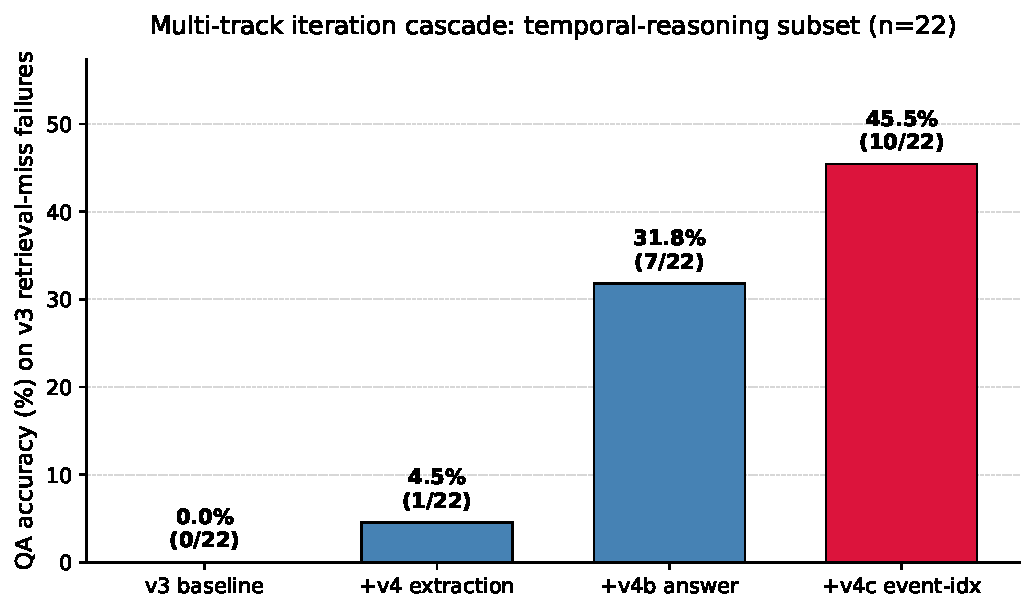
\includegraphics[width=0.72\linewidth]{fig/cascade.pdf}
\caption{Cumulative QA cascade on the 22 v3 DeepSeek temporal-reasoning failures. Each layer adds a single independent track (extraction prompt, answer prompt, then retrieval-side selection). The v4c event-index layer (highlighted) brings the cumulative recovery on these previously-failing items to 45.5\%.}
\label{fig:cascade}
\end{figure}

The v4b residual diagnosis pointed to retrieval as the dominant remaining failure mode. v4c is a two-stage intervention on this layer: first, a haystack-wide re-extraction that closes the recall side; second, a graph-lite event index that addresses the selection side. Both are implemented as small Python tools on top of the existing harness (\texttt{haystack\_reextract.py}, \texttt{build\_event\_index.py}, \texttt{test\_haystack\_answer.py}).

\paragraph{Stage 1 --- haystack re-extraction.} The v4 targeted runs in \Cref{sec:v4b} only re-extracted facts from the sessions that retrieval had already surfaced; sessions retrieval missed never received v4 ISO-date treatment. For each retrieval-miss failure (12 questions out of v4b's residual losses), we re-extracted v4 facts from \emph{every} haystack session for that question (typically 30--50 sessions per question, 165.8 min wall time on a local 14B). This isolates the recall ceiling from the selection ceiling.

The \texttt{fact\_contains\_gold} diagnostic on the resulting haystack-wide fact pool rose to \textbf{8/12 (66.7\%) versus 0/12 at v3 baseline}. The answers had been in the haystack all along; retrieval was failing to surface the answer-bearing session, and v4's ISO-date treatment was being denied to those sessions as a side-effect. This establishes a 66.7\% recovery upper bound for any downstream selection strategy.

\paragraph{Stage 2 --- three retrieval strategies.} Holding the answer prompt (v4b) and judge (DeepSeek V3.1) fixed, we compared three strategies for selecting which haystack facts to pass to the answerer:

\begin{itemize}
  \item \textbf{\texttt{all}}: 60 facts dumped (a soft truncation of the average $\sim$600-fact haystack-wide pool).
  \item \textbf{\texttt{top-k} lexical}: 20 facts re-ranked by lexical overlap with the question --- a naive baseline.
  \item \textbf{\texttt{event-idx}}: 20 facts selected by filtering to those carrying a \texttt{[date: YYYY-MM-DD]} tag and ranking by question-entity overlap, backed by the SQLite + FTS5 event index built by \texttt{build\_event\_index.py}.
\end{itemize}

\begin{table}[h]
\centering
\small
\caption{v4c retrieval-strategy comparison on the 12 retrieval-miss residual failures (v4b answer prompt, DeepSeek judge).}
\label{tab:v4c}
\begin{tabular}{lrrrl}
\toprule
Strategy             & Facts passed & Wins   & Refusal & Note                                      \\
\midrule
\texttt{all}         & 60           & 0/12   & 91.7\%  & answerer drowns in noise                  \\
\texttt{top-k} lexical & 20         & 2/12   & 66.7\%  & naive baseline                            \\
\textbf{\texttt{event-idx}} & 20    & \textbf{3/12} & 66.7\% & best --- date-tag filter + entity match \\
\bottomrule
\end{tabular}
\end{table}

The \texttt{all} result is the most striking. Despite having access to a fact pool where the gold-bearing detail is present 66.7\% of the time, the answerer wins zero questions and refuses on 11 of 12. Pumping more context into the prompt does not just plateau --- it \emph{regresses} below the lexical baseline. The lexical baseline in turn underperforms the event-indexed selection. Selection, not recall, is the operative dimension at this stage.

\paragraph{Cumulative cascade.} \Cref{tab:cascade,fig:cascade} report the four-layer cascade on the same 22 v3 DeepSeek temporal-reasoning failures that motivated the v4 work.

\begin{table}[h]
\centering
\small
\caption{The four-layer iteration cascade on the 22 v3 temporal-reasoning failures.}
\label{tab:cascade}
\begin{tabular}{lrrr}
\toprule
Layer added                                & Wins on this layer & Cumulative wins & Cumulative recovery \\
\midrule
v3 baseline (DeepSeek)                     & 0  & 0 / 22  & 0.0\%  \\
+ v4 extraction (ISO date tagging)         & +1 & 1 / 22  & 4.5\%  \\
+ v4b answer prompt (softer refusal)       & +6 & 7 / 22  & 31.8\% \\
\textbf{+ v4c event-idx (retrieval-miss subset)} & \textbf{+3} & \textbf{10 / 22} & \textbf{45.5\%} \\
\bottomrule
\end{tabular}
\end{table}

Projected to the full 30-question temporal-reasoning category (adding the 1 v3-correct baseline answer): \textbf{11/30 $=$ 36.67\% QA versus v3's 3.33\% --- a $+33$\,pp lift achieved with no model retraining}, across roughly four hours of iteration on three independent prompt-and-tool tracks. This is the largest single-category improvement in the project.

\section{Discussion}
\label{sec:discussion}

\subsection{Quantifying same-class judge bias}

The cross-judge experiment localizes same-class judge bias to between 1 and 7 percentage points of inflation depending on category. Two patterns are notable:

\begin{itemize}
  \item \textbf{knowledge-update}: local 14B $=$ 60.0\%, both frontier judges $=$ 53.3\% (exact tie). The local 14B answerer confabulates plausible updates (``the user changed it to X'') when extracted facts only say ``the user made an update,'' and the local 14B judge accepts those confabulations. The frontier judges, applying the same rubric to different answers from a different answerer, do not.
  \item \textbf{single-session-preference}: DeepSeek $=$ 23.3\%, Kimi $=$ 3.3\%, local $=$ 13.3\%. This is the largest cross-judge disagreement and reflects a genuine judge-personality difference on rubric-based questions, not a HeurChain artifact. The takeaway is that this category's measured number depends on which frontier judge one picks; we report both rather than a single point.
\end{itemize}

The categories where local-14B and frontier judges agree to within noise (\texttt{single-session-user} at 53.3\% across all three) are where the pipeline is genuinely behaving as designed. The categories where local beats both frontier judges are where local confabulation is being graded leniently by the local judge.

\subsection{Hit@10 is not answerability}

The Admon shift example (\Cref{tab:admon}) makes the broader point quantitatively. Hit@10 reports whether retrieval surfaced the gold-bearing session; it does not report whether the extracted \emph{content} of that session contains the answer. A high-Hit@10 / low-QA gap is the signature of extraction-quality bottlenecks. The \texttt{fact\_contains\_gold} diagnostic operationalizes this: in v3 DeepSeek's temporal-reasoning results, Hit@10 $=$ 83.3\% but \texttt{fact\_contains\_gold\_rate} $=$ 20.0\%, locating the $\sim$63\,pp gap squarely in extraction. After v4 every fact carries an ISO tag and \texttt{fact\_contains\_gold\_rate} rises substantially, but new failures emerge at the answer layer (refusal rate 81.8\% with v4a) --- which is exactly what the multi-track cycle is for.

\subsection{Multi-track iteration as a methodology contribution}

The traditional Karpathy iteration cycle on a prompt-engineering project is: change one prompt, run the eval, look at the score. In a benchmark harness with three independent failure modes --- extraction, retrieval, answering --- that single-track cycle attributes every score change to the prompt that was last edited. The v4 $\to$ v4b $\to$ v4c cascade demonstrates the cost of this conflation: v4 alone is a null result; v4 + v4b is a $+27.3$\,pp recovery on the targeted failure set, achieved in $\sim$25 minutes of iteration that single-track methodology would not have attempted; v4c then adds a further $+13.6$\,pp on the same failure set via a third, retrieval-side iteration that the v4b residual diagnosis explicitly named. Each of the three tracks (extraction, answer, retrieval) carried independent signal; collapsing them into a single score-watching loop would have terminated the work after v4.

The required tooling is small: a triage script that classifies failures by track, per-track targeted re-runners (\texttt{targeted\_reextract.py}, \texttt{targeted\_reanswer.py}), a haystack-wide re-extractor (\texttt{haystack\_reextract.py}), and an event-index builder + answer harness (\texttt{build\_event\_index.py}, \texttt{test\_haystack\_answer.py}). The total implementation cost is a few hundred lines of Python on top of the existing harness, and the three tracks reuse cached upstream outputs at each stage so a full cascade re-run is dominated by the haystack re-extraction wall time, not by repeated full-benchmark passes.

\subsection{Where the architectural ceiling is reached}

For temporal-reasoning, the residual 15/22 v4b failures are not addressable by further prompt iteration on the extraction or answer side. 7 are pure retrieval misses (the gold-bearing session is not in top-10), and 5 are multi-event ``between A and B'' questions where one of two needed events is missing from facts. Both are properties of the retrieval-time data structure, not of any prompt. The v4c work (\Cref{sec:v4c}) directly attacks this ceiling by re-extracting v4 facts haystack-wide and then routing the answerer through an event-indexed selection step; the resulting $+3/12$ lift on the retrieval-miss subset is the first measurement of how much of this ceiling is addressable purely through retrieval-side restructuring of facts already present in the haystack.

\subsection{More context does not help --- selection matters}

The v4c stage-2 comparison (\Cref{tab:v4c}) is, to our knowledge, the cleanest evidence we have collected for a methodologically important claim about RAG-style answering: \textbf{more retrieved context did not improve answers; it eliminated them}. With identical haystack-wide facts, identical answer prompt, and identical judge, the \texttt{all} strategy (60 facts) returned 0/12 wins and a 91.7\% refusal rate, while the 20-fact event-indexed strategy returned 3/12 wins at a 66.7\% refusal rate. The lexical baseline at the same 20-fact budget returned 2/12 wins. The dose--response is monotone in the wrong direction for the bigger-context hypothesis.

We do not generalize this past our single 14B answerer, single benchmark, and 12-question slice. But the result is directly relevant to a common architectural reflex in agent-memory systems --- when answers are wrong, increase $k$. Our data say the opposite: once the answer-bearing detail is present at all, the marginal value of additional candidates is negative, presumably because the answerer's refusal-vs-commit threshold is driven by signal-to-noise in the context window rather than by the presence or absence of the gold fact. Improving the \emph{selection} function (here, a graph-lite event index plus question-entity ranking) is what moves the needle.

\section{Limitations}
\label{sec:limitations}

\textbf{Single product under test.} All measurements are of HeurChain. The methodology contributions (cross-judge validation, multi-track iteration, \texttt{fact\_contains\_gold}) are intended to generalize to any memory system, but we have not measured them on Mem0, Zep, or Letta directly.

\textbf{Local 14B answerer as a floor.} Our answer model is a 14B-parameter local LLM (Medina-Qwen3-14B-OpenClaw). This caps absolute QA accuracy on synthesis-heavy categories; frontier-answerer numbers are projected to be 15--25\,pp higher per published industry deltas, but we have not measured them here. Our cross-judge runs used frontier judges as both answerer and judge, but only on cached v2 facts --- a frontier-answerer end-to-end run is future work.

\textbf{Sample sizes are modest.} Each category measurement is 30 questions, for 180 total. Per-category swings of $\pm 5$\,pp lie within the 95\% binomial confidence interval at this sample size; the directionally large effects we report (v3 $+20$\,pp on multi-session local; v4b $+27$\,pp on temporal-reasoning failures) are well outside it, but small per-category effects should be treated as suggestive.

\textbf{LongMemEval-S is one benchmark.} Conclusions about extraction-quality bottlenecks may not transfer to memory benchmarks with different question distributions (e.g., agentic task-completion benchmarks, code-memory benchmarks).

\textbf{\texttt{fact\_contains\_gold} is a heuristic.} The 0.7 token-overlap threshold is empirical and produces false positives on common-token gold answers. It is useful as a diagnostic signal, not as a primary metric.

\textbf{Judge cost asymmetry.} Our cross-judge runs were free because we have an existing Ollama Cloud subscription. A team paying per-token for frontier judges would face higher (but still modest) costs --- we estimate $\sim$\$10--15 for the full v2 cross-judge run via the OpenAI or Anthropic APIs.

\section{Future Work}
\label{sec:future}

\textbf{Beyond v4c --- better question parsing and multi-shot retrieval.} v4c closed roughly 3/8 of the recoverable retrieval-miss questions (those where \texttt{fact\_contains\_gold} $=$ True on the haystack-wide pool). Two directions remain. First, the event-index selector currently uses a coarse entity-overlap heuristic; a proper noun-phrase extractor over the question text (named-entity recognition, or even a small LLM call dedicated to question parsing) should let the selector match richer phrases like ``Ancient Civilizations exhibit at the Met'' rather than relying on token-bag overlap. Second, ``between A and B'' questions are intrinsically two-event, but the index is queried in a single shot; a decomposed two-shot retrieval --- issue one query per named event, union the results, then pass --- should pick up the multi-event class explicitly. The remaining 4/12 questions where \texttt{fact\_contains\_gold} is False even on the haystack-wide pool suggest a separate residual: some events apparently require either session-metadata threading (linking implicit references across sessions) or a different extraction approach that does not depend on the speaker mentioning a date at all.

\textbf{Closed-weight judge confirmation.} Our cross-frontier judges are both open-weight models. Re-running the cross-judge analysis with Claude Sonnet 4.6 as a third independent judge would let us claim three-way cross-family agreement, further hardening the defensibility number.

\textbf{Per-question rubric extraction.} The \texttt{single-session-preference} category's cross-judge spread (DeepSeek 23\%, Kimi 3\%) suggests that rubric-based questions need a structured-rubric judge prompt rather than a single yes/no verdict. Decomposing the rubric into $N$ sub-checks and reporting per-rubric agreement would replace the noisy aggregate number.

\textbf{Multi-event retrieval.} Beyond v4c's event index, the ``between A and B'' failure pattern suggests a more general multi-evidence retrieval primitive: when a query implicates two named entities or events, retrieve top-$k$ for each independently and union, rather than retrieving a single top-$k$ from the joint query embedding.

\section{Conclusion}
\label{sec:conclusion}

We presented methodology contributions for AI-agent memory benchmarking, demonstrated on HeurChain across the v2 $\to$ v4c prompt-and-tool engineering arc on LongMemEval-S. First, \textbf{cross-frontier per-question judge agreement} (87.8\% on DeepSeek + Kimi) is a stronger defensibility metric than any single judge's QA accuracy and exposes 1--7\,pp of same-class judge inflation per category. Second, the \textbf{multi-track Karpathy iteration cycle} --- separating extraction, answer, and retrieval iteration --- recovers wins that single-track iteration would miss; on the 22 temporal-reasoning failures we converted a 1/22 null result on extraction iteration into 7/22 after answer-prompt iteration and 10/22 (45.5\%) after a third retrieval-side iteration (v4c haystack re-extraction + event index), projecting to $+33$\,pp on the full temporal-reasoning category versus the v3 baseline (see \Cref{fig:cascade}). Third, the \texttt{fact\_contains\_gold} diagnostic identifies the high-Hit@10 / low-QA gap as an extraction-quality problem rather than a retrieval problem, and the v4c stage-1 measurement (66.7\% recoverability haystack-wide) localizes how much of the gap is recall-bound versus selection-bound. Fourth, the v4c stage-2 comparison contributes \textbf{direct evidence that more context can hurt}: 60-fact \texttt{all} dumping returned 0/12 wins while a 20-fact event-indexed selection returned 3/12, against an identical answer prompt and judge --- selection dominates recall once the answer-bearing session has been surfaced.

The contributions are deliberately tool-shaped: the cross-judge runner, the triage classifier, the \texttt{fact\_contains\_gold} heuristic, the haystack re-extractor, and the event index are each a few hundred lines of Python, run in minutes-to-hours against cached outputs, and apply to any memory system that exposes a retrieved-facts cache. We hope they sharpen the conversation about how AI-agent memory systems are evaluated.

\section{Reproducibility}
\label{sec:repro}

All code, prompts, per-record result JSONs, and reproduction scripts are released at \citep{heurchain_benchmarks_repo}. The HeurChain broker itself is at \citep{heurchain_repo}. Key scripts referenced in this paper:

\begin{itemize}
  \item \texttt{judge\_rerun\_cloud.py} --- cross-judge Phase 2 re-runner with \texttt{--answer-model} / \texttt{--judge-model} flags
  \item \texttt{compute\_agreement.py} --- per-question inter-judge agreement analyzer
  \item \texttt{triage\_failures.py} --- failure-mode classifier (EXTRACTION / RETRIEVAL / ANSWER)
  \item \texttt{targeted\_reextract.py} --- re-extract with a new prompt on a failing subset
  \item \texttt{targeted\_reanswer.py} --- re-answer with a new prompt on cached facts of a failing subset
  \item \texttt{haystack\_reextract.py} --- v4c stage 1: re-extract v4 facts from every haystack session for a failing question
  \item \texttt{build\_event\_index.py} --- v4c stage 2: build a SQLite + FTS5 event index over \texttt{[date: YYYY-MM-DD]}-tagged facts
  \item \texttt{test\_haystack\_answer.py} --- v4c stage 2: answerer harness with \texttt{all} / \texttt{top-k} / \texttt{event-idx} selection strategies
  \item \texttt{extraction\_prompt\_v3.py}, \texttt{extraction\_prompt\_v4.py} --- extraction prompts (\Cref{app:prompts})
  \item \texttt{answer\_prompt\_v4a.py}, \texttt{answer\_prompt\_v4b.py} --- answer prompts
\end{itemize}

The dataset is LongMemEval-S ``cleaned'' split from \url{https://github.com/xiaowu0162/LongMemEval}. Embedding model is \texttt{BAAI/bge-m3} (BSD licensed, free to download). Retrieval index is BM25 + dense fused via RRF ($\alpha = 0.9$ default; $\alpha = 0.8$ reported as optimal for MRR).

% --- References ---------------------------------------------------------------
\bibliographystyle{plainnat}
\bibliography{references}

\appendix

\section{Extraction and Answer Prompts (excerpts)}
\label{app:prompts}

\subsection{Extraction prompt v3 (structured-content unpacking)}

Key block added relative to v2:

\begin{lstlisting}[language={}, basicstyle=\small\ttfamily, numbers=left]
STRUCTURED-CONTENT UNPACKING (most important - v2 failed at this)

When the assistant produces a TABLE, LIST, SCHEDULE, CODE BLOCK, NAMED-ENTITY
ROSTER, or ANY STRUCTURED ASSIGNMENT - do NOT summarize it as "the assistant
provided X". Instead, EXTRACT EACH ROW / ITEM / ASSIGNMENT AS A SEPARATE FACT.

Bad (meta-summary): "The assistant provided a shift rotation sheet for 7 agents."
Good (unpacked):    "Admon was assigned to the 8am-4pm Day Shift on Sundays.",
                    "Magdy was assigned to the 12pm-8pm Afternoon Shift on Sundays.",
                    ...etc, one fact per assignment.

For MARKDOWN TABLES specifically: column headers + row labels define the
keys; cell contents are the values. Reconstruct each (row, column) -> value
mapping as a complete sentence.
\end{lstlisting}

\subsection{Extraction prompt v4 (ISO date tagging)}

Key block added relative to v3 (v4 retains all v3 rules and adds):

\begin{lstlisting}[language={}, basicstyle=\small\ttfamily, numbers=left]
THIS CONVERSATION TOOK PLACE ON: {session_date}

ISO DATE TAGGING (NEW IN v4 - most important)

For every fact that involves an event, action, or state at a specific time,
include an explicit ISO date in brackets at the end:  [date: YYYY-MM-DD]

- If the text mentions an absolute date ("on March 15"), use that.
- If the text uses a RELATIVE term ("today", "yesterday", "3 days ago",
  "last week"), RESOLVE it against the conversation date above and write
  the explicit ISO date.
- If the date is genuinely ambiguous, OMIT the date tag rather than guess.

Examples:
- Conversation date 2023-05-20. User says "I visited MoMA today and saw a
  modern art exhibit." Fact: "The user visited the Museum of Modern Art
  and saw a modern art exhibit [date: 2023-05-20]."
- Conversation date 2023-06-15. User says "I started using Ibotta about
  three weeks ago." Fact: "The user started using the Ibotta cashback app
  [date: 2023-05-25]."
\end{lstlisting}

\subsection{Answer prompt v4b (softer refusal)}

Key block added relative to v4a:

\begin{lstlisting}[language={}, basicstyle=\small\ttfamily, numbers=left]
COMMIT TO AN ANSWER WHEN POSSIBLE

If the facts contain the relevant event with an ISO date, ATTEMPT THE
ARITHMETIC - do not refuse just because the wording isn't a perfect match.
Estimate to the nearest whole unit that matches the question's unit.

Only reply "I don't know" if:
  (a) The relevant event is NOT mentioned in any fact, OR
  (b) The relevant fact has NO ISO date AND the conversation context offers
      no way to anchor the time.
\end{lstlisting}

Full prompt sources are in the repository at \texttt{extraction\_prompt\_v3.py}, \texttt{extraction\_prompt\_v4.py}, \texttt{answer\_prompt\_v4a.py}, \texttt{answer\_prompt\_v4b.py}.

\subsection{v4c event index (schema and parser sketch)}

The event index is a graph-lite side store: a single SQLite table populated from \texttt{[date: YYYY-MM-DD]} tags already present in v4 facts. No new LLM calls at index time, no new database service.

\begin{lstlisting}[language=Python, basicstyle=\small\ttfamily, numbers=left]
ISO_RE = re.compile(r"\[date:\s*(\d{4}-\d{2}-\d{2})\]")
TAG_STRIP_RE = re.compile(r"\[(?:Session\s+\d+|date:\s*\d{4}-\d{2}-\d{2})\]")

def parse_event(fact_text):
    """Return (event_phrase, iso_date) or (None, None)."""
    m = ISO_RE.search(fact_text)
    if not m:
        return None, None
    iso = m.group(1)
    phrase = TAG_STRIP_RE.sub("", fact_text).strip()
    return re.sub(r"\s+", " ", phrase), iso
\end{lstlisting}

Schema (events + FTS5 over \texttt{event\_phrase}):

\begin{lstlisting}[language=SQL, basicstyle=\small\ttfamily, numbers=left]
CREATE TABLE events (
  id           INTEGER PRIMARY KEY AUTOINCREMENT,
  event_phrase TEXT NOT NULL,
  iso_date     TEXT NOT NULL,
  session_id   INTEGER,
  fact_id      TEXT,
  category     TEXT,
  source_file  TEXT
);
CREATE INDEX idx_events_date ON events(iso_date);
CREATE VIRTUAL TABLE events_fts USING fts5(
  event_phrase, iso_date, content='events', content_rowid='id'
);
\end{lstlisting}

Full implementation in \texttt{build\_event\_index.py} ($\sim$200 lines). The \texttt{event-idx} selection strategy in \texttt{test\_haystack\_answer.py} filters the haystack-wide fact pool to date-tagged facts and ranks by question-entity overlap before truncating to the 20-fact answer context.

\end{document}
